We generalize the work of \citet{dong15} to the multi-task sequence-to-sequence
learning setting that includes the tasks of machine translation (MT),
constituency parsing, and image caption generation. Depending which tasks 
involved, we propose to categorize multi-task \ssl{} learning into three general
settings.
In addition, we will discuss the unsupervised learning tasks considered as well
as the learning process.

\paragraph{One-to-Many Setting}
%\label{subsec:otm}
This scheme involves {\it one encoder} and {\it multiple decoders} for tasks in
which the encoder can be shared, as illustrated in
Figure~\ref{f:otm}. The input to each task is a sequence of
English words. A separate decoder is used to generate each sequence of
output units which can be either (a) a sequence of tags for
constituency parsing as used in \citep{vinyals15grammar}, (b) a
sequence of German words for machine translation \citep{luong15attn},
and (c) the same sequence of English words for autoencoders or a
related sequence of English words for the skip-thought objective
\citep{kiros15skip}.

\begin{figure}[tbh]
\centering
%\psgrid
%\rput(7.5,2.6){$\alpha_1=1.0$}
%\rput(7.5,1.5){$\alpha_2=0.1$}
%\rput(7.5,0.4){$\alpha_3=0.5$}
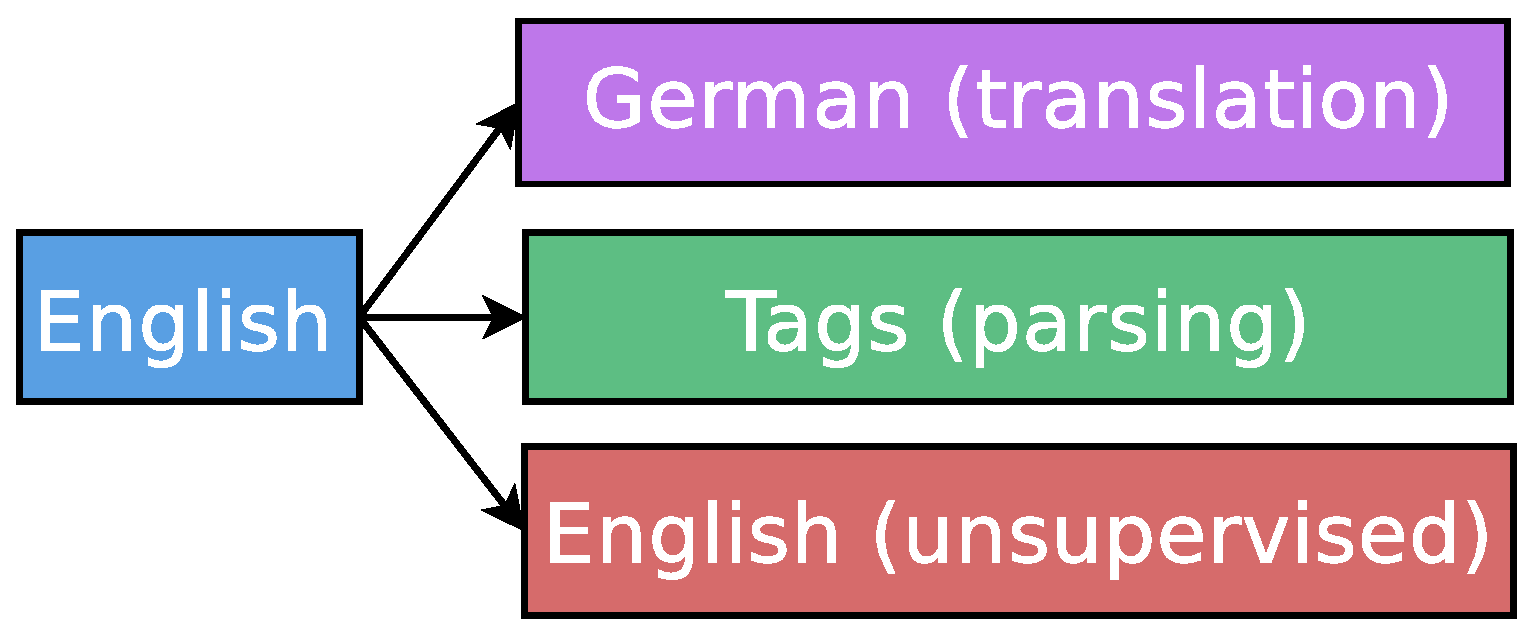
\includegraphics[width=0.45\textwidth, clip=true, trim= 0 0 0
0]{img/6-1_otm}
\caption{{\bf One-to-many Setting} -- one encoder, multiple decoders. This scheme
is useful for either multi-target translation as
in \cite{dong15} or between different tasks. Here, English and
German imply sequences of words in the respective languages. 
%The $\alpha$ values
%give the proportions of parameter updates that are allocated for the different tasks.
} 
\label{f:otm}
\end{figure}

\paragraph{Many-to-One Setting}
%\label{subsec:mto}
This scheme is the opposite of the {\it one-to-many}
setting. As illustrated in Figure~\ref{f:mto}, it consists of {\it multiple
encoders} and {\it one decoder}. This is useful for tasks in which only the
decoder can be shared, for example, when our tasks include machine translation
and image caption generation \citep{vinyals15caption}. In addition, from a machine
translation perspective, this setting can benefit from a large
amount of monolingual data on the target side, which is a standard
practice in machine translation system and has also been explored
for neural MT by \cite{gulcehre2015using}.

\begin{figure}[tbh]
\centering
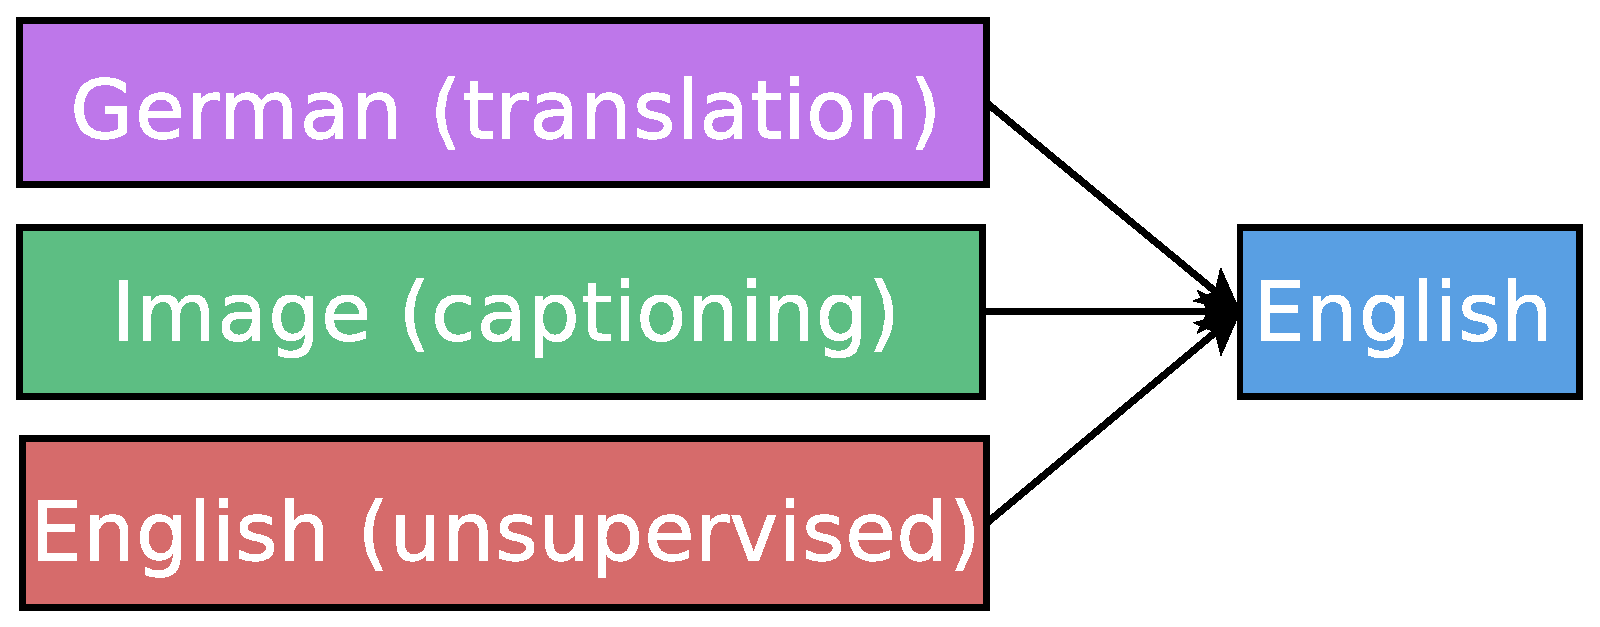
\includegraphics[width=0.5\textwidth, clip=true, trim= 0 0 0
0]{img/6-1_mto}
\caption{{\bf Many-to-one setting} -- multiple encoders, one decoder. This scheme
is handy for tasks in which only the decoders can be shared.}
\label{f:mto}
\end{figure}

\paragraph{Many-to-Many Setting}
%\label{subsec:mtm}
Lastly, as the name describes, this category is the most general one,
consisting of multiple encoders and multiple decoders.
%However, such
%flexibility also makes it difficult to determine which tasks should
%share which components. ---- Is it true? IS. 
%To simplify sharing, we consider a special use
%case in machine translation which involves two encoders and two
%decoders shared over three tasks.
We will explore this scheme in a translation setting that involves sharing multiple
encoders and multiple decoders.  In addition to the machine
translation task, we will include two unsupervised 
objectives over the source and target languages as illustrated in
Figure~\ref{f:mtm}.

\begin{figure}[tbh]
\centering
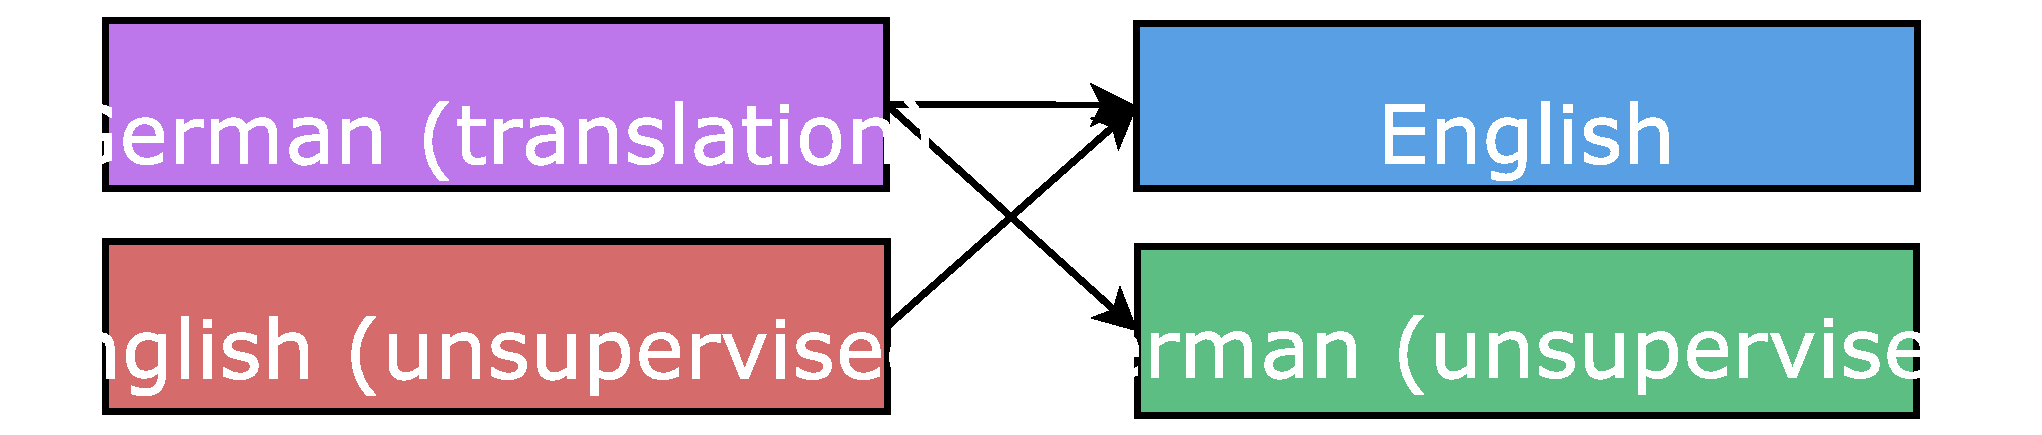
\includegraphics[width=0.7\textwidth, clip=true, trim= 0 0 0
0]{img/6-1_mtm}
\caption{{\bf Many-to-many setting} -- multiple encoders, multiple decoders. We
consider this scheme in a limited context of machine translation to utilize the large
monolingual corpora in both the source and the target languages. Here, we
consider a single translation task and two unsupervised autoencoder tasks.} 
\label{f:mtm}
\end{figure}

\paragraph{Unsupervised Learning Tasks}

Our very first unsupervised learning task involves learning {\it autoencoders} from
monolingual corpora, which has recently been applied to sequence to sequence
learning \citep{dai15}. However, in \citet{dai15}'s work, the authors
only experiment with pretraining and then finetuning, but not joint training which
can be viewed as a form of multi-task learning (MTL). As such, we are
very interested in knowing whether the same trend extends to our MTL settings.

Additionally, we investigate the use of the {\it skip-thought}
vectors \citep{kiros15skip} in the context of our MTL framework.
Skip-thought vectors are trained by training sequence to sequence
models on pairs of consecutive sentences, which makes the skip-thought
objective a natural \ssl{} learning candidate. A minor technical
difficulty with skip-thought objective is that 
the training data must consist of ordered sentences, e.g., paragraphs.  Unfortunately, in
many applications that include machine translation, we only have
sentence-level data where the sentences are unordered. To
address that, we split each sentence into two halves; we then use 
one half to predict the other half.

\paragraph{Learning}
%\label{subsec:learning}
\cite{dong15} adopted an {\it alternating} training approach, where they
optimize each task for a fixed number of parameter updates (or
mini-batches) before switching to the next task (which is a different
language pair). In our setting, our tasks are more diverse and contain
different amounts of training data. As a result, we allocate different
numbers of parameter updates for each task, which are expressed with
the {\it mixing} ratio values $\alpha_i$ (for each task $i$). Each
parameter update consists of training data from one task only. When
switching between tasks, we select randomly a new task $i$ with
probability $\frac{\alpha_i}{\sum_j \alpha_j}$.
%{\bf [Thang, make sure that it is correct]} 


Our convention is that the first task is the
{\it reference} task with $\alpha_1 = 1.0$ and the number of training
parameter updates for that task is prespecified to be $N$. A typical task $i$ will then be
trained for $\frac{\alpha_i}{\alpha_1}\cdot N$ parameter updates.
Such convention makes it easier for us to fairly compare the same reference
task in a single-task setting which has also been trained for exactly $N$
parameter updates.

When sharing an encoder or a decoder, we share both the recurrent connections
and the corresponding embeddings.

%This ensures
%fairness when comparing the performance of the reference task trained
%alone using the same number of mini-batches.
%IS:  I don't think that it follows.


